\documentclass[UTF8]{article}
% Template based on https://www.overleaf.com/latex/templates/assignment-template/fwycphfzpshm

\usepackage[authoryear]{natbib}
\usepackage{url}
\usepackage{amsmath}
\usepackage{amsfonts}
\usepackage[margin=1in]{geometry}
\usepackage{multirow}
\usepackage{graphicx}
\usepackage{pdfpages}

\title{AttentiveCLS Pooler}
\author{
  Team 1:  % team no
  Seungil Lee, Jongchan Park, Eugene Seo, and Dohyung Kim % your names
}
\date{\today}

\begin{document}
\maketitle

\section{Introduction}

BERT~\cite{devlin-etal-2019-bert} has become a standard architecture for NLP research ever since it was published. BERT computes the representation for every token, but it uses the output representation of the special token \texttt{[CLS]}, for sentence-level tasks (e.g., sentiment analysis). However, various strategies were introduced to get sentence-level representation.

We have designed new pooler named \texttt{AttentiveCLS} pooler and evaluated its performance on CoLa, MNLI, RTE and SST-2 tasks, which are the representatives of sentence-level tasks. The results were compared with \texttt{MeanMaxTokens} pooler, which is suggested in the homework description, also with the original \texttt{BERTPooler} in \texttt{huggingface} library (\url{https://huggingface.co/}).

\section{AttentiveCLS Pooler}
Though original BERT pooler simply adopts last output of \texttt{[CLS]} token, we tried to exploit information from other tokens as well. Nowadays, attention mechanism is widely used to get the importance of the given sequence, so we added a attention pooling layer on the top of the tokens other than \texttt{[CLS]} token. Then, the output of this attention layer is concatenated with the last output of \texttt{[CLS]} token. We also apply linear transformation with $W \in \mathbb{R}^{H \times 2H}$ and $\tanh$ activation just like as the \texttt{BERTPooler} in \texttt{huggingface} implementation.

\begin{figure}[htp] \centering{
  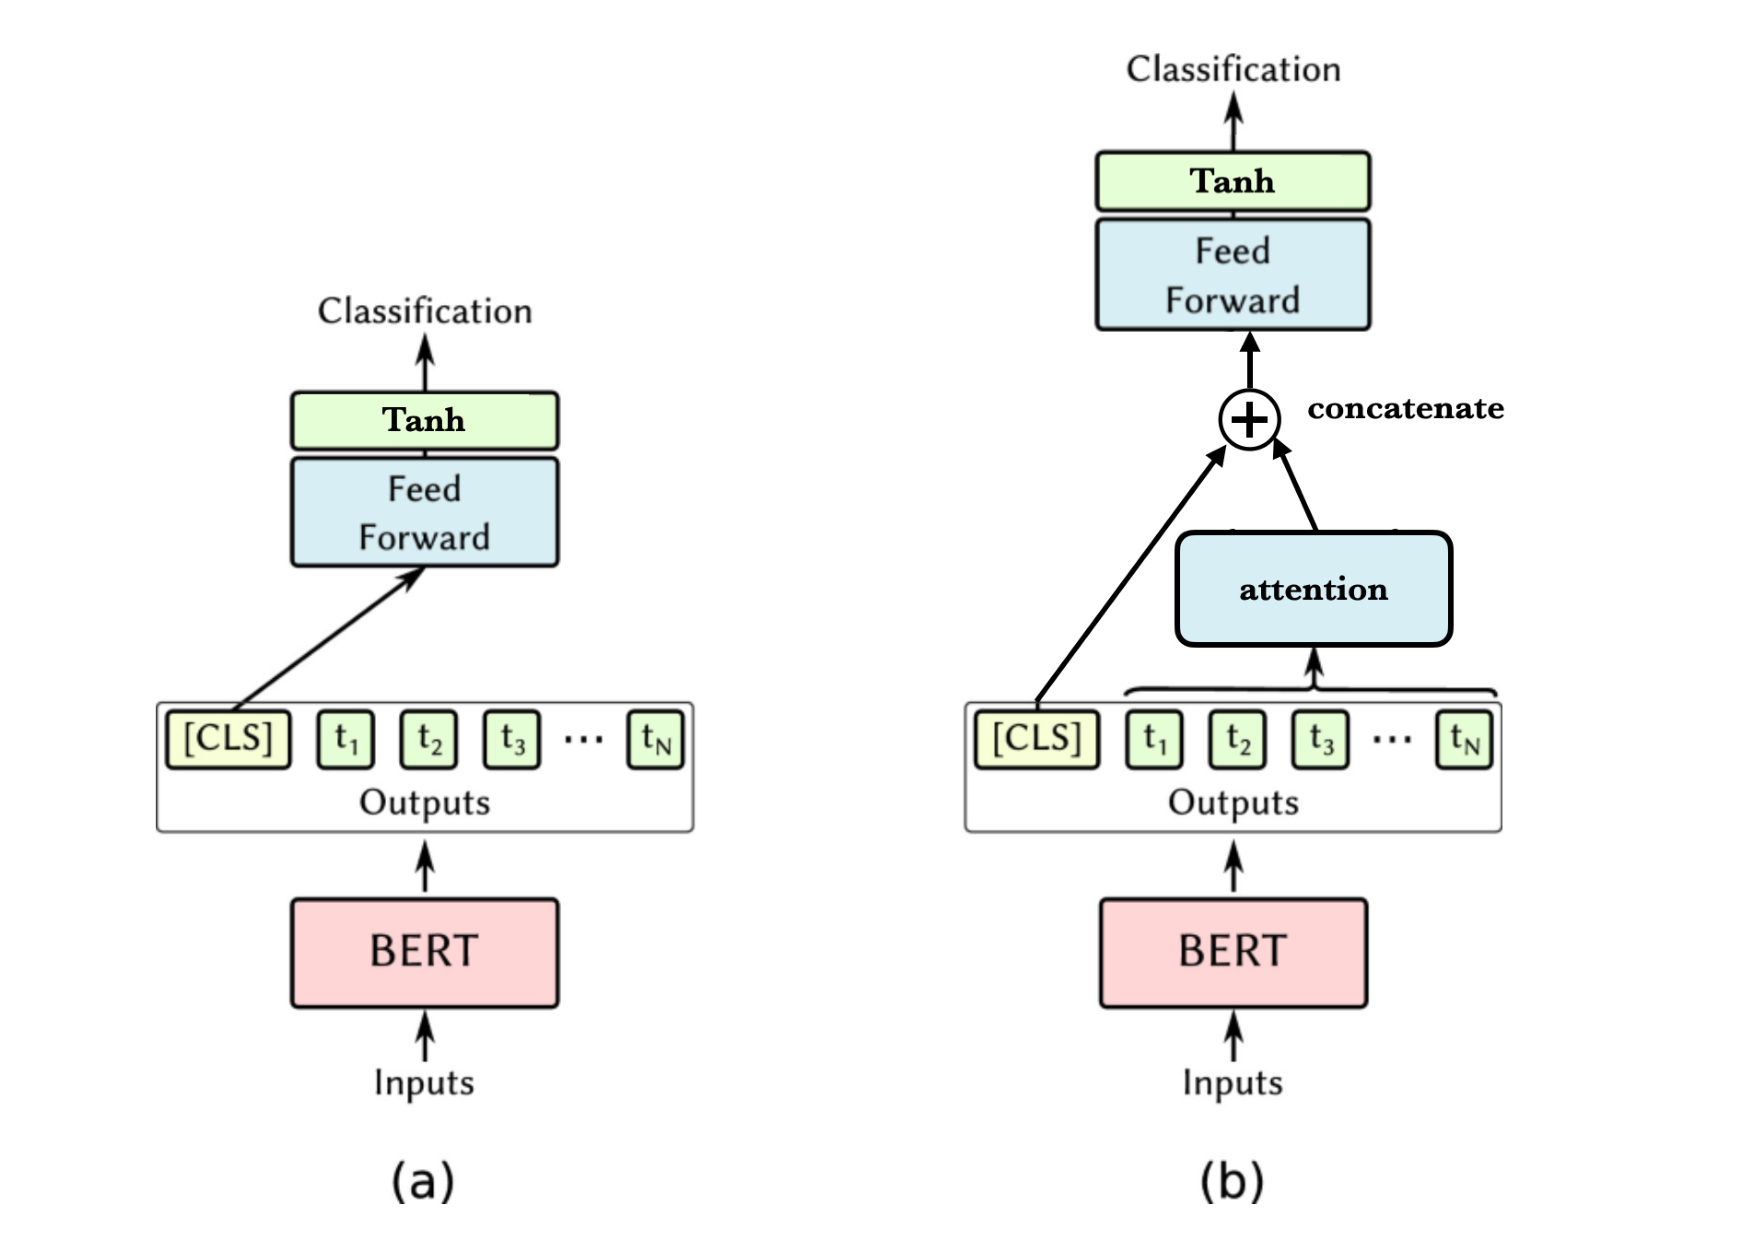
\includegraphics[scale=0.4]{figure1.pdf}}
  \caption{Schematic visualization of AttentiveCLS. This figure is modified from the paper~\cite{lehevcka2020adjusting}}
  \end{figure} 


\section{Result}

\begin{table}[h]
  \resizebox{\textwidth}{!}{%
  \begin{tabular}{|l|ll|lll|ll|ll|}
  \hline
  \multirow{2}{*}{} & \multicolumn{2}{l|}{CoLA}                                   & \multicolumn{3}{l|}{MRPC}                                                                     & \multicolumn{2}{l|}{RTE}                               & \multicolumn{2}{l|}{SST-2}                             \\ \cline{2-10}
  & \multicolumn{1}{l|}{Loss}            & Matthews & \multicolumn{1}{l|}{Accuracy}        & \multicolumn{1}{l|}{F1}              & Loss            & \multicolumn{1}{l|}{Accuracy}        & Loss            & \multicolumn{1}{l|}{Accuracy}        & Loss            \\ \hline
  AttentiveCLS      & \multicolumn{1}{l|}{0.4588}          & \textbf{0.6044}      & \multicolumn{1}{l|}{\textbf{0.8544}} & \multicolumn{1}{l|}{\textbf{0.9012}} & \textbf{0.3952} & \multicolumn{1}{l|}{0.6137}          & 0.7498          & \multicolumn{1}{l|}{0.9289}          & 0.3272          \\ \hline
  MeanMax           & \multicolumn{1}{l|}{\textbf{0.4208}} & 0.5375               & \multicolumn{1}{l|}{0.8162}          & \multicolumn{1}{l|}{0.8777}          & 0.4424          & \multicolumn{1}{l|}{0.5379}          & \textbf{0.6920} & \multicolumn{1}{l|}{\textbf{0.9312}} & 0.2711          \\ \hline
  BERTPooler        & \multicolumn{1}{l|}{0.4388}          & 0.5934               & \multicolumn{1}{l|}{0.8456}          & \multicolumn{1}{l|}{0.8934}          & 0.4000          & \multicolumn{1}{l|}{\textbf{0.6462}} & 0.7058          & \multicolumn{1}{l|}{0.9300}          & \textbf{0.2387} \\ \hline
  \end{tabular}%
  }
  \caption{Table showing the result of 4 experiments. Bold numbers indicate the best performance among 3 poolers.}
  \label{tab:result}
  \end{table}


In this experiment, we use 4 different text classification tasks (CoLA, MRPC, RTE, SST-2) in the GLUE~\cite{wang2018glue} benchmark to evaluate 3 pooler strategies. Each dataset has its own evaluation metrics (e.g. Accuracy, F1).

Table \ref{tab:result} shows our experiment results. 
For CoLA task, AttentiveCLS results highest performance for Matthews correlation and MeanMax has the best performance for loss value.
Interestingly, for MRPC task, AttentiveCLS is superior to other strategies for all evaluation metrics. 
However, for RTE and SST-2 tasks, AttentiveCLS doesn’t have the highest performance for any metrics. 
For RTE task, BERTPooler has the best accuracy and MeanMax has the best loss value. 
On the other hand, for SST-2 task, MeanMax has the best accuracy and BERTPooler has the best loss value.

This result shows that each pooler can show different performance depending on the dataset. 
In our dataset, AttentiveCLS has good performance on most metrics. Interestingly, only AttentiveCLS shows the best performance for all metrics in the specific dataset(MRPC).


\bibliographystyle{plain}
\bibliography{report.bib}


\end{document}
